\documentclass[12pt]{article}

%==============================
%        PACOTES BÁSICOS
%==============================
\usepackage[utf8]{inputenc}
\usepackage[T1]{fontenc}
\usepackage[brazil]{babel}
\usepackage[useregional]{datetime2}
\usepackage{graphicx}
\usepackage{amsmath, amssymb}
\usepackage{setspace}
\usepackage{enumitem}
\usepackage[colorlinks=true, linkcolor=black, urlcolor=blue, citecolor=black]{hyperref}
\usepackage{caption}
\usepackage{parskip}
\usepackage{float}
\usepackage{ragged2e}
\usepackage{helvet}
\renewcommand{\familydefault}{\sfdefault}
\usepackage{titlesec}
\usepackage[a4paper, top=2cm, bottom=2.5cm, left=3cm, right=2cm]{geometry}
\usepackage{tcolorbox}

\usepackage{tikz}
\usetikzlibrary{circuits.logic.US}

\usepackage{tabularx}
\usepackage{array, xcolor, booktabs}
\usepackage[table]{xcolor}
\usepackage{multirow}

%==============================
%      INDENTAÇÃO ABNT
%==============================
\usepackage{indentfirst}
\setlength{\parindent}{1.25cm}

%==============================
%      ESTILO DAS SECTIONS
%==============================
%gostaria que tivesse com o /newpage no final automático

%==============================
%        DOCUMENTO
%==============================
\begin{document}

%==============================
%            CAPA
%==============================
\begin{titlepage}
\thispagestyle{empty}
\centering

{\large Escola Politécnica da Universidade de São Paulo\par}
\vspace{1.2em}

{\large \textbf{PCS3115} -- Sistemas Digitais I (2026)\par}
\vspace{5em}

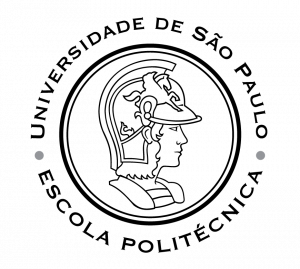
\includegraphics[width=0.4\textwidth]{logo.png}
\vspace{4em}

{\Large\bfseries Ralatório da Atividade Formativa I\par}
\vspace{4em}

{\Large Turma: 1/3\par}
Professor(es): Antonio Vieira da Silva Neto

\vfill

\begin{center}
Victor Augusto D M N da Silva (NUSP: 16903351)\\
Nome 2 (NUSP: XXXXXXXX)\\
Nome 3 (NUSP: XXXXXXXX)
\end{center}

\vspace{1em}
{\large São Paulo, \the\year\par}

\end{titlepage}

%==============================
%          SEÇÕES
%==============================
\section{Exercício 1 - Sistemas de numeração, código e aritmética}

\begin{tcolorbox}[title=Enunciado da Questão,colback=gray!5,colframe=black]

Em um jogo que envolve batalhas entre personagens, como os pertencentes às
franquias \textit{Super Mario RPG} e \textit{Pokémon}, fórmulas matemáticas
atreladas às características dos personagens em conflito são utilizadas para
determinar o dano causado por um golpe e se ele é suficiente, ou não, para que
o oponente seja derrotado.

Considere um jogo assemelhado a esses, no qual cada personagem possui um
nível que determina sua vida e um conjunto de golpes. Cada golpe $k$ de um
personagem $X$ possui uma força $G_{X,k}$ e pode ser utilizado por até
$n_{X,k}$ vezes em uma batalha.

Dessa forma, quando um golpe $k$ é utilizado, a quantidade $n_{X,k}$ é
diminuída em uma unidade, e quando $n_{X,k} = 0$, o golpe fica bloqueado
pelo restante da batalha.

Quando um personagem $A$ desfere um golpe de força $G_{A,k}$ em um
personagem $B$, o golpe sempre acerta seu alvo.Dessa forma, a vida do personagem $B$ é diminuída de $G_{A,k}$, tal como
definido na Equação~(\ref{eq:dano}):

\begin{equation}
\text{Vida}_B = \text{Vida}_B - G_{A,k}
\label{eq:dano}
\end{equation}

A mecânica do jogo é plenamente reflexiva e vale, portanto, igualmente
para golpes do personagem $B$ em direção ao personagem $A$.
Por fim, um personagem é derrotado quando sua vida for menor ou igual
a zero após receber um golpe.

Em um protótipo preliminar do jogo \textit{Super Mario RPG}, é realizada
uma batalha-teste entre dois personagens: ``Geno'', controlado por um
jogador humano, e ``Yaridovich'', que segue uma programação do próprio jogo.
Nesse teste, assuma as seguintes características para os personagens
e seus golpes.

\textbf{Geno}
\begin{itemize}
\item Vida: $67$
\item Golpe 1 (Finger Shot): $G_{G,1}=2$, $n_{G,1}=58$
\item Golpe 2 (Hand Gun): $G_{G,2}=5$, $n_{G,2}=7$
\item Golpe 3 (Geno Blast): $G_{G,3}=46$, $n_{G,3}=1$
\end{itemize}

\textbf{Yaridovich}
\begin{itemize}
\item Vida: $79$
\item Golpe 1 (Pierce): $G_{Y,1}=3$, $n_{Y,1}=29$
\item Golpe 2 (Flame Stone): $G_{Y,2}=10$, $n_{Y,2}=3$
\item Golpe 3 (Water Blast): $G_{Y,3}=27$, $n_{Y,3}=1$
\end{itemize}

\end{tcolorbox}

\subsection{Pergunta (a)}

\subsubsection*{Enunciado}

Considere que os cálculos de decremento unitário de $n_{x,k}$ e da Equação~(1)
sejam realizados em base binária no hardware do jogo, e assuma que nenhum
dos atributos envolvidos --- $G_{x,k}$, $n_{x,k}$ e $\text{Vida}$ --- tenha
módulo superior a $127$.

Quais devem ser as quantidades mínimas de bits para representar cada um
desses atributos?

\subsubsection*{Resposta}
A primeira consideração que fizemos foi que quando a pergunta se refere à quantidade mínima de bits do jogo, ele esteja se referindo a todas as situações possíveis do jogo limitadas pela condição que ele estipulou e não o caso específico do Genos e Yaridovich.

Dessa forma, como $G_{x,k}$ e $n_{x,k}$ representam quantidades não negativas com
valor máximo de $127$, precisamos de um número de bits capaz de
representar valores no intervalo $[0,127]$. Em binário, seria: $127_{10} = 1111111_2$ e ,portanto, são necessários \textbf{7 bits} para representar esses valores.

Já o atributo $\text{Vida}$ pode assumir valores negativos, logo deve ser representado com os mesmos algarismos para o módulo e um sinal (em complemento de dois), pois com $8$ bits em complemento de dois é possível representar o intervalo

\[
-128 \leq x \leq 127
\]

Assim, as quantidades mínimas de bits são:

\begin{itemize}
\item $G_{x,k}$: $7$ bits
\item $n_{x,k}$: $7$ bits
\item $\text{Vida}$: $8$ bits
\end{itemize}

\subsection{Pergunta (b)}

\subsubsection*{Enunciado}

Preencha a Tabela~\ref{tab:batalha} mostrando, em bases binária e
hexadecimal, os valores das vidas dos personagens ``Geno'' e
``Yaridovich'' na batalha descrita até que um personagem vença.

Indique até que linha da tabela o jogo efetivamente ocorrerá e
justifique sua resposta mostrando os cálculos da forma como são
feitos no jogo, isto é, executando as operações na base binária.

\subsubsection*{Resposta}
As vidas iniciais são representadas em $8$ bits com sinal e a evolução das vidas ao longo da batalha é apresentada na
Tabela~\ref{tab:batalha} considerando que:

\begin{itemize}
\item Geno: $67_{10} = 01000011_2 = 43_{16}$
\item Yaridovich: $79_{10} = 01001111_2 = 4F_{16}$
\end{itemize}

\newcolumntype{Y}{>{\centering\arraybackslash}X}

\begin{table}[H]
\small
\centering
\caption{Sequência de Jogadas de Batalha entre Geno e Yaridovich}
\label{tab:batalha}

\renewcommand{\arraystretch}{1.3}

\begin{tabularx}{\textwidth}{
|>{\centering\arraybackslash}m{0.8cm}
|>{\centering\arraybackslash}m{5.5cm}
|>{\centering\arraybackslash}X
|>{\centering\arraybackslash}X
|>{\centering\arraybackslash}X
|>{\centering\arraybackslash}X|}

\hline
\rowcolor{gray!25}
 & &
\textbf{Binário} &
\textbf{Hex} &
\textbf{Binário} &
\textbf{Hex} \\
\cline{3-6}

\rowcolor{gray!25}
\multirow{-2}{*}{\textbf{Linha}} &
\multirow{-2}{*}{\textbf{Ação}} &
\multicolumn{2}{c|}{\textbf{Vida Geno}} &
\multicolumn{2}{c|}{\textbf{Vida Yaridovich}} \\
\hline

0 & Início da Batalha (Vida Completa) &
01000011 & 43 &
01001111 & 4F \\
\hline

1 & Geno usa ``Geno Blast'' $(G=46)$ &
01000011 & 43 &
00100001 & 21 \\
\hline

2 & Yaridovich usa ``Water Blast'' $(G=27)$ &
00101000 & 28 &
00100001 & 21 \\
\hline

3 & Geno usa ``Hand Gun'' $(G=5)$ &
00101000 & 28 &
00011100 & 1C \\
\hline

4 & Yaridovich usa ``Flame Stone'' $(G=10)$ &
00011110 & 1E &
00011100 & 1C \\
\hline

5 & Geno usa ``Hand Gun'' $(G=5)$ &
00011110 & 1E &
00010111 & 17 \\
\hline

6 & Yaridovich usa ``Flame Stone'' $(G=10)$ &
00010100 & 14 &
00010111 & 17 \\
\hline

7 & Geno usa ``Hand Gun'' $(G=5)$ &
00010100 & 14 &
00010010 & 12 \\
\hline

8 & Yaridovich usa ``Flame Stone'' $(G=10)$ &
00001010 & 0A &
00010010 & 12 \\
\hline

9 & Geno usa ``Hand Gun'' $(G=5)$ &
00001010 & 0A &
00001101 & 0D \\
\hline

10 & Yaridovich usa ``Pierce'' $(G=3)$ &
00000111 & 07 &
00001101 & 0D \\
\hline

11 & Geno usa ``Hand Gun'' $(G=5)$ &
00000111 & 07 &
00001000 & 08 \\
\hline

12 & Yaridovich usa ``Pierce'' $(G=3)$ &
00000100 & 04 &
00001000 & 08 \\
\hline

13 & Geno usa ``Hand Gun'' $(G=5)$ &
00000100 & 04 &
00000011 & 03 \\
\hline

14 & Yaridovich usa ``Pierce'' $(G=3)$ &
00000001 & 01 &
00000011 & 03 \\
\hline

15 & Geno usa ``Hand Gun'' $(G=5)$ &
00000001 & 01 &
11111110 & Morto \\
\hline

16 & Yaridovich usa ``Pierce'' $(G=3)$ &
 &  &
 &  \\
\hline

17 & Geno usa ``Finger Shot'' $(G=2)$ &
 &  &
 &  \\
\hline

18 & Yaridovich usa ``Pierce'' $(G=3)$ &
 &  &
 &  \\
\hline

19 & Geno usa ``Finger Shot'' $(G=2)$ &
 &  &
 &  \\
\hline

20 & Yaridovich usa ``Pierce'' $(G=3)$ &
 &  &
 &  \\
\hline

21 & Geno usa ``Finger Shot'' $(G=2)$ &
 &  &
 &  \\
\hline

22 & Yaridovich usa ``Pierce'' $(G=3)$ &
 &  &
 &  \\
\hline

\end{tabularx}
\end{table}

Na linha 15, Geno utiliza o golpe ``Hand Gun'' $(G=5)$.
O cálculo realizado em aritmética binária de 8 bits é:

\[
00000011_2 - 00000101_2 = 11111110_2
\]

Em complemento de dois, $11111110_2 = -2_{10}$. Assim,
$\text{Vida}_{Yaridovich} \le 0$ e Yaridovich é derrotado nessa jogada.

Portanto, a batalha termina na linha 15 da tabela e as linhas
seguintes permanecem sem valores de vida, pois o jogo não
prossegue após a derrota de um personagem.

\subsection{Pergunta (c)}
\subsubsection*{Enunciado}

O que ocorreria na batalha se, seguindo a mesma sequência de golpes da Tabela~\ref{tab:batalha}, Yaridovich fosse o primeiro a atacar? Quais seriam as vidas de Geno e Yaridovich no final dessa variante de conflito? Justifique sua resposta.

\subsubsection*{Resposta}

Se Yaridovich fosse o primeiro a atacar, mantendo-se a mesma sequência de golpes da Tabela~\ref{tab:batalha}, a ordem das ações seria apenas deslocada: o primeiro ataque seria de Yaridovich, seguido pelo ataque inicial de Geno, e assim sucessivamente.

No início da batalha, Geno possui 67 pontos de vida e Yaridovich possui 79 pontos de vida. Caso Yaridovich inicie o combate utilizando o golpe ``Water Blast'' $(G=27)$, a vida de Geno seria reduzida imediatamente para 40 pontos.

Em seguida, Geno utilizaria ``Geno Blast'' $(G=46)$, reduzindo a vida de Yaridovich para 33 pontos. A partir desse ponto, a sequência de golpes continua exatamente como descrita na tabela.

Entretanto, como Geno passa a receber dano antes de executar seu primeiro ataque, ele sofre um ataque adicional de Yaridovich ao longo da sequência. Considerando que Geno termina a sequência original com apenas 1 ponto de vida, esse ataque extra faria sua vida atingir um valor negativo antes que pudesse realizar o golpe final.

Portanto, nessa variante da batalha, Geno seria derrotado primeiro, enquanto Yaridovich ainda permaneceria com vida positiva no momento da derrota do oponente. Assim, inverter a ordem inicial dos ataques altera o resultado final do combate, resultando na vitória de Yaridovich.

\subsection{enunciado para (d) e (e)}
\begin{tcolorbox}[title=Enunciado da Questão,colback=gray!5,colframe=black]

Como a exibição de números decimais para o usuário final do jogo é mais intuitiva,
em função do uso da base decimal nas escolas e em nosso cotidiano ``não técnico'' —
algo que você deve ter vivenciado até as aulas anteriores —, as informações de vida,
força de golpes e quantidade de ataques devem ser apresentadas na tela utilizando
um código BCD (Binary-Coded Decimal).

Nesse código, cada dígito decimal (de 0 a 9) é representado por um conjunto de bits
binários.

Em relação ao código BCD e ao seu uso no jogo, responda:

\end{tcolorbox}

\subsection{Pergunta (d)}

\subsubsection*{Enunciado}
Quantos bits são necessários para representar um dígito decimal? Por quê?

\subsubsection*{Resposta}
Para representar um dígito decimal no código BCD são necessários \textbf{4 bits}.

Isso ocorre porque um dígito decimal pode assumir \textbf{10 valores possíveis}
(0 a 9). Com $n$ bits é possível representar $2^n$ combinações diferentes.
Assim, precisamos encontrar o menor valor de $n$ tal que:

\[
2^n \geq 10
\]

Testando os valores:

\[
2^3 = 8 < 10
\]

\[
2^4 = 16 \geq 10
\]

Logo, são necessários \textbf{4 bits} para representar um dígito decimal em BCD.
Nesse código, cada dígito de 0 a 9 é representado por um grupo de 4 bits.
Por exemplo:

\[
0 = 0000 \quad
5 = 0101 \quad
9 = 1001
\]

As combinações restantes (1010 até 1111) não são utilizadas no código BCD.

\subsection{Pergunta (e)}

\subsubsection*{Enunciado}
Quantos bits são necessários para representar os atributos
$G_{x,k}$, $n_{x,k}$ e Vida? Considere que, além de o módulo de todos eles
ser limitado a 127, valores negativos de Vida são sempre limitados a ``0''
na tela para o usuário final.

Exemplifique mostrando os valores binários, em BCD, das especificações de
$G_{x,k}$, $n_{x,k}$ e Vida do personagem Yaridovich antes de qualquer
confronto.

\subsubsection*{Resposta}
Como o valor máximo possível dos atributos é 127, o maior número decimal
a ser representado possui três dígitos.

No código BCD cada dígito decimal é representado por 4 bits. Portanto,
para representar um número de até três dígitos são necessários:

\[
3 \times 4 = 12 \text{ bits}
\]

Assim, os atributos $G_{x,k}$, $n_{x,k}$ e Vida devem ser representados
com \textbf{12 bits em BCD}.

Antes de qualquer confronto, o personagem Yaridovich possui:

\[
Vida = 79, \qquad G_{x,k} = 10, \qquad n_{x,k} = 8
\]

Convertendo para BCD:

\[
79 = 0111\ 1001
\]

\[
10 = 0001\ 0000
\]

\[
8 = 0000\ 1000
\]

Cada grupo de 4 bits representa um dígito decimal independente.

\section{Exercício 2 - Eletrônica digital CMOS}
\begin{tcolorbox}[title=Enunciado da Questão,colback=gray!5,colframe=black]

Considere o circuito da Figura~\ref{fig:circuito_derrota}, utilizado para
implantar uma parte da lógica de detecção de derrota de um personagem no
contexto do Exercício~1.

Na figura, os sinais do tipo $\text{Vida[MSB]}(k)$ e $\text{Vida[MSB]}(k+1)$
representam o bit mais significativo (MSB -- \textit{Most Significant Bit})
da vida do personagem nas jogadas $k$ e $k+1$, respectivamente.

O sinal \textit{Saída} é igual a ``1'' estritamente quando a situação de
derrota é satisfeita.

Considerando o circuito da Figura 1, responda as questões subsequentes.

\end{tcolorbox}

\begin{figure}[H]
\centering
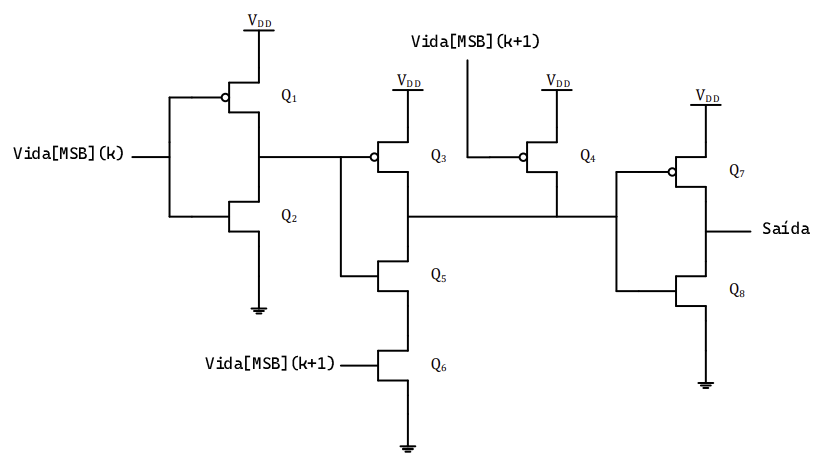
\includegraphics[width=0.9\textwidth]{circuitoEx2.png}
\caption{Circuito de detecção de derrota.}
\label{fig:circuito_derrota}
\end{figure}

\subsection{Pergunta (a)}

\subsubsection*{Enunciado}
Qual a expressão lógica do sinal \textit{Saída} em função de
$\text{Vida[MSB]}(k)$ e 
$\text{Vida[MSB]}(k+1)$?

\subsubsection*{Resposta}

A lógica do circuito detecta a transição do bit mais significativo da vida
de $0$ para $1$, o que indica que o valor da vida tornou-se negativo após a
jogada.

\textbf{Tabela-verdade}

\begin{table}[H]
\centering
\renewcommand{\arraystretch}{1.3}
\begin{tabular}{|c|c|c|}
\hline
$\text{Vida[MSB]}(k)$ & $\text{Vida[MSB]}(k+1)$ & Saída \\
\hline
0 & 0 & 0 \\
0 & 1 & 1 \\
1 & 0 & 0 \\
1 & 1 & 0 \\
\hline
\end{tabular}
\end{table}

\textbf{Representação lógica equivalente}

A função pode ser implementada utilizando um inversor seguido de uma porta
AND.

\begin{center}
\begin{tikzpicture}[circuit logic US, every circuit symbol/.style={scale=1}]

\node (A) at (0,1) {$\text{Vida[MSB]}(k)$};
\node (B) at (0,-1) {$\text{Vida[MSB]}(k+1)$};

\node[not gate, draw, logic gate inputs=nn] (not1) at (2,1) {};
\node[and gate, draw, logic gate inputs=nn] (and1) at (4,0) {};

\draw (A) -- (not1.input);
\draw (not1.output) -- (and1.input 1);

\draw (B) -- (and1.input 2);

\draw (and1.output) -- (6,0) node[right]{Saída};

\end{tikzpicture}
\end{center}

Assim, a saída deve ser ativada quando:

\[
\text{Vida[MSB]}(k) = 0 \ \ \ e \ \ \ \text{Vida[MSB]}(k+1) = 1
\]

Portanto, a expressão lógica do sinal de saída pode ser escrita como

\[
\text{Saída} = \overline{\text{Vida[MSB]}(k)} \cdot \text{Vida[MSB]}(k+1)
\]

\subsection{Pergunta (b)}

\subsubsection*{Enunciado}

Explique qual parte da lógica de detecção de derrota de um personagem
esse circuito implanta.

\subsubsection*{Resposta}

Como os valores são representados em complemento de dois, o bit mais
significativo indica o sinal do número. Assim, quando o MSB passa de
$0$ para $1$, isso significa que o valor da vida tornou-se negativo.

O circuito, portanto, detecta exatamente essa transição o momento em que a vida do personagem
passa de um valor não negativo para um valor negativo após a aplicação
de um golpe e ativa o sinal
de saída quando ela ocorre, indicando que a condição de derrota foi
atingida.

\subsection{Pergunta (c)}

\subsubsection*{Enunciado}

O que ocorreria com a lógica implantada pelo circuito da Figura~1 se,
por uma falha aleatória, a conexão da porta (G) do transistor Q2 ficar
em aberto? Assuma que nenhuma outra falha ocorra ao mesmo tempo.

\subsubsection*{Resposta}

Se a porta do transistor Q2 ficar em aberto, o seu estado lógico torna-se
indefinido, pois a tensão no terminal de controle não estará fixada em
nenhum nível lógico específico.

Nesse caso, o transistor pode conduzir ou permanecer desligado de forma
imprevisível devido a ruídos elétricos ou acoplamentos parasitas.

Como consequência, o comportamento da primeira etapa lógica do circuito
torna-se indeterminado, podendo gerar valores incorretos na saída
intermediária e, consequentemente, ativar ou desativar o sinal de derrota
de forma errática.

\subsection{Pergunta (d)}

\subsubsection*{Enunciado}

O que ocorreria com a lógica implantada pelo circuito da Figura~1 se,
por uma falha aleatória, houvesse curto-circuito na junção dreno-fonte
(D-S) do transistor Q6? Assuma que nenhuma outra falha ocorra ao mesmo
tempo que ela.

\subsubsection*{Resposta}

Se ocorrer um curto-circuito entre o dreno e a fonte do transistor Q6,
o caminho para o terra permanecerá permanentemente conectado.

Assim, o nó controlado por esse transistor será forçado ao nível lógico
baixo independentemente do valor aplicado à sua porta.

Como consequência, a lógica implementada pelo circuito ficará alterada,
podendo impedir que o sinal de saída atinja o nível lógico alto mesmo
quando a condição de derrota for satisfeita, ou causar um comportamento
incorreto na detecção dessa condição.


\subsection{Pergunta (e)}

\subsubsection*{Enunciado}
Qual deve ser a expressão lógica necessária para implantar a segunda parte da lógica de detecção de derrota de um personagem? Explique sua resposta fazendo um esboço do esquema elétrico de um circuito CMOS que a implante e calcule a quantidade mínima de transistores para implantá-la, assumindo que não haja limitações elétricas (i.e., sem limites por fan-in ou fan-out).

\subsubsection*{Resposta}

A segunda parte da lógica de detecção de derrota deve identificar quando a
vida do personagem torna-se igual a zero. Considerando uma representação
binária de $n$ bits

\[
V_{n-1} V_{n-2} \dots V_0
\]

a condição $\text{Vida}=0$ ocorre somente quando todos os bits são iguais a
zero. Logo, a função lógica correspondente pode ser escrita como:

\[
Z = \overline{V_{n-1} + V_{n-2} + \dots + V_0}
\]

Essa função é equivalente a uma porta NOR de $n$ entradas.

\bigskip

\textbf{Esboço do circuito lógico}

\begin{center}
\begin{tikzpicture}[circuit logic US]

\node (nor) at (3,0) [nor gate, draw, logic gate inputs=nnn] {};

\node (v2) at (0,0.8) {$V_{n-1}$};
\node (v1) at (0,0) {$V_{n-2}$};
\node (vd) at (0,-0.8) {$\dots$};
\node (v0) at (0,-1.6) {$V_0$};

\draw (v2) -- (nor.input 1);
\draw (v1) -- (nor.input 2);
\draw (v0) -- (nor.input 3);

\draw (nor.output) -- (5,0) node[right]{Vida = 0};

\end{tikzpicture}
\end{center}

\bigskip

\textbf{Implementação CMOS}

Uma porta NOR de $n$ entradas em CMOS é implementada com:

\begin{itemize}
\item $n$ transistores PMOS em série na rede de pull-up
\item $n$ transistores NMOS em paralelo na rede de pull-down
\end{itemize}

Assim, a quantidade mínima de transistores necessária é:

\[
2n
\]

Para o caso do exercício, em que a vida é representada com $8$ bits:

\[
2 \times 8 = 16 \text{ transistores}
\]

Portanto, a segunda parte da lógica de detecção de derrota pode ser
implantada com uma porta NOR de $n$ entradas, utilizando $2n$
transistores em CMOS.

\end{document}